\documentclass[parskip=full,11pt,twoside]{scrartcl}
\usepackage[utf8]{inputenc}

\title{VIPER: Viper Interactive Prolog Education Runtime}
\subtitle{Pflichtenheft}
\author{Paul Brinkmeier, Lukas Brocke, Jannik Koch, Aaron Maier, Christian Oder}

% section numbers in margins:
\renewcommand\sectionlinesformat[4]{\makebox[0pt][r]{#3}#4}

% header & footer
\usepackage{scrlayer-scrpage}
\lofoot{\today}
\refoot{\today}
\pagestyle{scrheadings}

\usepackage{amsmath} % for $\text{}$

\usepackage[sfdefault,light]{roboto}
\usepackage[T1]{fontenc}
\usepackage[german]{babel}
\usepackage[yyyymmdd]{datetime} % must be after babel
\renewcommand{\dateseparator}{-} % ISO8601 date format
\usepackage{hyperref}
\usepackage[nameinlink]{cleveref}
\crefname{figure}{Abb}{Abb}
\usepackage[section]{placeins}
\usepackage{xcolor}
\usepackage{graphicx}
\usepackage{listings}
\usepackage{courier}
\hypersetup{
	pdftitle={Pflichtenheft},
}

\usepackage{csquotes}

\newcommand\urlpart[2]{$\underbrace{\text{\texttt{#1}}}_{\text{#2}}$}

\usepackage{pflichtenheft}

\lstset{basicstyle=\ttfamily,breaklines=true}

% Don't strech across whole page
\raggedbottom

% Start new page with each section
\usepackage{sectsty}
\sectionfont{\clearpage}

\begin{document}
\maketitle

\section{Einleitung}

Prolog ist eine logische Programmiersprache die ein deklaratives Programmieren ermöglicht.

Prolog operiert auf einer Wissensdatenbank, deren Einträge sich Fakten und Regeln nennen. Ein Beispiel:

\begin{lstlisting}
father(abe, homer).
father(homer, bart).
\end{lstlisting}

So gilt, dass Abe der Vater von Homer und Homer der Vater von Bart ist.

Für eine Abfrage erhalten wir folgende Lösungen:

\begin{lstlisting}
?- father(homer, bart).
yes .
?- father(bart, abe).
no .
\end{lstlisting}

Nun ist es möglich, auf Fakten basierende Regeln einzuführen. Definieren wir also Großväter väterlicherseits als alle Väter von Vätern, indem wir Variablen als Platzhalter verwenden. Diese beginnen mit Großbuchstaben, Funktoren und Atome mit Kleinbuchstaben.

\begin{lstlisting}
paternalGrandfather(X, Y) :- father(X, Z), father(Z, Y).
\end{lstlisting}

Selbiges ist möglich für Abfragen.

\begin{lstlisting}
?- father(X, bart).
X = homer .
?- father(X, Y).
X = homer, Y = bart ;
X = abe, Y = homer .
?- paternalGrandfather(X, Y).
X = abe, Y = bart .
\end{lstlisting}

Die Antworten sind alle möglichen Kombinationen aus den Variablen, die den Fakten und Regeln entsprechen.

Prolog ist hierbei anders als \enquote{andere} Programmiersprachen, da es sich um eine deklarative Programmiersprache handelt. Imperative Programmiersprachen (bspw. die Programmiersprache C) erledigen sequentiell eine vorgeschriebene Reihenfolge von Befehlen. Damit steht der Prozess des Lösens im Vordergrund. Deklarative Programmiersprachen wie Prolog beschreiben ein Problem und ermitteln den Lösungsweg automatisch. Im Vordergrund steht hier hingegen die Problembeschreibung.

Zur Lösung eines Problems nutzt Prolog das Konzept der Unifikation. Dazu werden verschiedene Belegungen getestet, welche unter Umständen keine gültige Lösung sind. Im Falle ungültiger Lösungen wird die letzte Entscheidung zur Belegung rückgängig gemacht (\enquote{Backtracking}) und die nächste Belegung getestet.

VIPER, die VIPER Interactive Prolog Education Runtime, ist ein Programm zur Bearbeitung und dem Testen von einfachen Prolog-Programmen. Über die visuelle Schnittstelle ist es dem Nutzer möglich, Prolog zu schreiben, Abfragen zu stellen und die Abarbeitung dieser visualisieren zu lassen.

Die Visualisierung für einzelne Schritte der Interpretation ist hierbei als gerichteter Graph realisiert. Der genannte Graph entspricht einem Baum mit \enquote{Rückwärts-Kanten} (da einzelne Schritte visualisiert werden, gibt es jeweils höchstens eine Rückwärts-Kante pro Visualisierung-Schritt), die das Backtracking veranschaulichen.

Unter Zuhilfenahme der Visualisierung soll der Nutzer die Interpretation eines Prolog-Programms schrittweise nachvollziehen können. Dies soll dem Nutzer die Funktionsweise von Prolog-Programmen näher bringen und das Verständnis für die Eigenschaften der Sprache stärken.

\section{Kriterien}

\subsection{Muss}

\criterium{Erstellen eines neuen Prolog-Programms}{crt:create}

Das Programm stellt einen leeren Editor für neue Prolog-Programme bereit. Der Inhalt des Editors wird dabei gelöscht.

\criterium{Öffnen eines Prolog-Programms}{crt:open}

Das Programm kann bereits vorhandene Prolog-Programme öffnen.

\criterium{Bearbeiten eines Prolog-Programms}{crt:edit}

Das Programm erlaubt es dem Nutzer, Änderungen an einem geöffneten Prolog-Programm durchzuführen. Dabei wird die aktuelle Interpretation gestoppt und die Visualisierung gelöscht.

\criterium{Speichern eines Prolog-Programms}{crt:save}

Das Programm kann Änderungen am momentan geladenen Prolog-Programm speichern. Der Inhalt der Datei wird dabei überschrieben.

\criterium{Parsen eines Prolog-Programms mit begrenztem Sprachumfang}{crt:parser}

Das Programm kann eine Teilmenge der Sprache Prolog durch einen Parser verarbeiten.

\criterium{Eingabe von Abfragen}{crt:request}

Das Programm erlaubt es dem Nutzer Abfragen in das Eingabefeld einzugeben. Dabei wird die aktuelle Interpretation abgebrochen und die Visualisierung gelöscht.

\criterium{Einzelschritt-Interpretation von Abfragen}{crt:interpreter}

Das Programm bearbeitet Abfragen schrittweise. Nach jedem durchgeführten Teilschritt einer Abfrage wartet das Programm auf eine Interaktion vom Nutzer (Klicken der \enquote{Nächster Schritt}-Schaltfläche), bis es den nächsten Teilschritt bearbeitet.

\criterium{Visualisierung als Graph}{crt:visualization}

Das Programm kann die Abarbeitung einer Abfrage zu einem Prolog-Programm durch einen Graphen visualisieren.

\criterium{Ausgabe von Lösungen zu einer Abfrage}{crt:answer}

Das Programm kann Lösungen zu einer Abfrage in der Konsole ausgeben. Dabei wird bei einer Abfrage ohne Variablen \enquote{yes} oder \enquote{no} ausgegeben. Beinhaltet die Abfrage Variablen, so werden mögliche Variablenbelegungen ausgegeben. Gibt es keine Lösung, so wird eine entsprechende Meldung ausgegeben.

\subsection{Kann}

\criteriumOptional{Zurückschreiten}{crt:stepback}

Das Programm soll es dem Nutzer ermöglichen, beliebig viele Schritte schrittweise zurückzugehen.

\criteriumOptional{Ausführung bis zur nächsten Lösung}{crt:continue}

Die Interpretation soll durch eine zusätzliche Schaltfläche bis zur nächsten Lösung ausgeführt werden können. Diese Aktion kann durch das Betätigen der \enquote{Abbrechen}-Schaltfläche abgebrochen werden. Dabei wird der aktuelle Interpretationsschritt fertig berechnet und anschließend wird die Interpretation beendet.

\criteriumOptional{Cut}{crt:cut}

Das Programm soll die \enquote{Cut}-Funktionalität unterstützen.

\criteriumOptional{Arithmetik}{crt:maths}

Das Programm soll grundlegende Arithmetik unterstützen.

\criteriumOptional{Standardbibliothek}{crt:standardlib}

Das Programm soll eine Standardbibliothek mit nützlichen, vordefinierten Regeln unterstützen, die standardmäßig beim Starten des Programms mit eingebunden wird. Bereits implementierte Regeln, die vom Nutzer nochmals implementiert werden, werden als zusätzliche Regeln zu den bereits vorhandenen hinzugefügt nachdem eine Warnung ausgegeben wurde.

\criteriumOptional{Standardbibliothek deaktivieren und aktivieren}{crt:disablelib}

Das Programm soll es dem Nutzer ermöglichen, die eingebundene Standardbibliothek deaktivieren und wieder aktivieren zu können.

\criteriumOptional{Export von Visualisierungsbäumen als LaTeX-Code}{crt:latexexport}

Das Programm kann einen Visualisierungsbaum als LaTeX-Code exportieren, damit dieser vereinfacht in Dokumente eingebunden werden kann.

\criteriumOptional{Export von Visualisierungsbäumen als Bilddatei}{crt:imageexport}

Das Programm kann einen Visualisierungsbaum als Bilddatei im SVG- oder PNG-Format exportieren.

\criteriumOptional{\enquote{Pretty-Printing} von Listen}{crt:prettyprinting}

Das Programm soll Listen bei der Ausgabe einheitlich auf \enquote{\texttt{[x,y,z]}} formatieren.

\criteriumOptional{Formatierung von Quelltext}{crt:formatting}

Das Programm soll Quelltext durch das Betätigen der \enquote{Formatieren}-Schaltfläche in ein vorgeschriebenes Format bringen können.

\criteriumOptional{Wechseln der Sprache zwischen Deutsch und Englisch}{crt:translation}

Die Programmoberfläche soll die Sprachen Deutsch und Englisch unterstützen.

\subsection{Abgrenzung}

\criteriumNot{Voller Sprachsupport}{crt:fullsupport}

Das Programm unterstützt keine Prolog-Sprachfeatures außerhalb der vorgestellten Prolog-Teilmenge.

\criteriumNot{Andere Programmiersprachen}{crt:otherlanguages}

Das Programm beschränkt sich auf die Prolog-Sprache und bietet keine offizielle Unterstützung für Prolog-Dialekte oder andere Programmiersprachen jeglicher Art.

\criteriumNot{Nutzung in einer Kommandozeile}{crt:cli}

Das Programm beschränkt sich auf eine graphische Darstellung über GUI-Elemente. Eine Interaktion über die Konsole wird nicht unterstützt.

\criteriumNot{Professionelle Anwendung}{crt:professionaluse}

Das Programm ist nicht für professionelle Anwendungszwecke ausgelegt.

\criteriumNot{Parser}{crt:parser}

Der Parser ist gegeben und wird nicht selbst implementiert.

\section{Produkteinsatz}

Das Programm soll als graphisches Prolog-Lerntool betrieben werden.

Die Zielgruppe des Lerntools sind Lehrende, Studierende und Enthusiasten.

Das Programm soll sich auf eine Teilmenge der Prolog-Sprache beschränken, diese jedoch voll unterstützen.

Das Programm soll für die Teilmenge der Sprache eine Lernhilfe sein und das Verständnis für die Funktionsweise von Prolog, mit Hilfe von schrittweiser Visualisierung, stärken.

Das Programm ermöglicht es mit Hilfe eines eingebauten Editors Prolog-Programme zu bearbeiten und zu erweitern.

\section{Produktumgebung}

Das Programm soll als graphische Applikation auf einem Desktop-System betrieben werden.

Es stehen mindestens 2 AMD64/x86 Kerne mit insgesamt 2GB shared RAM zur Verfügung.

Unterstützte Betriebssysteme sind Windows ab Version 7 und aufwärts, macOS 10.9 aufwärts sowie Ubuntu Linux 16.04.

Eine Maus sowie eine Tastatur sind als Eingabegeräte angeschlossen und funktionsfähig.

Eine Installation des Java Runtime Environments Version 8 aufwärts ist auf dem System vorhanden.

\section{Produktdaten}

\textbf{Zuletzt geöffnete Dateien} \\
Die Pfade der fünf zuletzt geöffneten Dateien werden für einen Eintrag in der Menüleiste gespeichert.

Außer den oben genannten werden keinerlei Daten gespeichert.

\section{Funktionale Anforderungen}

\functionality{Erstellen eines neuen Prolog-Programms}{fnc:new}
\fulfills{crt:create}

Das Programm stellt einen Editor bereit, in dem ein leeres Prolog-Programm angelegt werden kann. Sollte der Editor zuvor bereits ungesicherten Inhalt besitzen, so wird der Nutzer aufgefordert, diesen zu speichern. Hierbei kann entweder die alte Datei überschrieben oder eine neue Datei angelegt werden. Der alte Inhalt wird daraufhin verworfen und ein neues Prolog-Programm angelegt.

\functionality{Öffnen eines Prolog-Programms}{fnc:open}
\fulfills{crt:open}

Das Programm ist in der Lage, Prolog-Programmdateien zu öffnen. Der Datei-Inhalt wird dabei in den Editor geladen und angezeigt. Analog wird zur Erstellung eines neuen Prolog-Programms, falls nötig, zur Speicherung ungesicherter Inhalte aufgefordert und das alte Prolog-Programm daraufhin verworfen.

\functionality{Öffnen eines zuletzt verwendeten Prolog-Programms}{fnc:recentfiles}
\fulfills{crt:open}

Das Programm bietet einen Schnellzugriff auf bis zu fünf der zuletzt verwendeten Dateien an. Diese können analog zu F2 geöffnet werden.

\functionality{Bearbeiten eines Prolog-Programms}{fnc:editor}
\fulfills{crt:edit}

Das Prolog-Programm kann im Editor bearbeitet werden. Die Änderungen werden erst beim Speichern zurückgeschrieben.

\functionality{Speichern als}{fnc:saveas}
\fulfills{crt:save}

Ist der Dateiname noch nicht durch das Öffnen eines bereits vorhandenen Prolog-Programms oder durch vorheriges Speichern bekannt, so kann über einen Auswahldialog eine neue Datei angelegt werden.

\functionality{Speichern des Editor-Inhalts}{fnc:save}
\fulfills{crt:save}

Das Programm kann den Inhalt des Editors speichern. Ist der Dateiname bekannt wird der Inhalt der Datei überschrieben. Sollte dies nicht der Fall sein wird die \enquote{Speichern als...} Funktion ausgeführt.

\functionality{Parsen eines Prolog-Programms}{fnc:parser}
\fulfills{crt:parser}
\fulfills{crt:standardlib}

Das geöffnete Prolog-Programm kann durch einen Parser verarbeitet werden. Wird der Parser gestartet, werden die Fenster der Konsole und der Visualisierung geleert.

\functionality{Fehlerausgabe beim Parsen eines inkorrekten Prolog-Programms}{fnc:errorcheck}
\fulfills{crt:parser}

Der Parser erkennt Fehler innerhalb des geöffneten Prolog-Programms bei der Verarbeitung. Fehlermeldungen werden über das verfügbare Konsolen-Fenster ausgegeben.

\functionality{Eingabe von Prolog-Abfragen in das Eingabefeld}{fnc:shell}
\fulfills{crt:request}

Bei erfolgreicher Verarbeitung einer korrekten Datei durch den Parser erlaubt das Eingabefeld die Eingabe von Abfragen. Sollten erneut Änderungen an dem geöffneten Prolog-Programm stattfinden, so wird das Eingabefeld deaktiviert sowie jegliche Interaktion mit der Visualisierung gesperrt bis der veränderte Quelltext erneut vom Parser verarbeitet wurde.

\functionality{Syntaktische Fehler in der Abfrage}{fnc:inputerror}
\fulfills{crt:request}

Syntaktische Fehler in der Abfrage werden in der Konsole ausgegeben.

\functionality{Interpretation von Prolog-Abfragen}{fnc:interpreter}
\fulfills{crt:interpreter}
\fulfills{crt:cut}
\fulfills{crt:maths}

Abfragen, welche im Eingabefeld eingegeben wurden, werden nach einer Bestätigung mit der Eingabe-Taste schrittweise interpretiert.

\functionality{Weiterschreiten in der Interpretation}{fnc:interpreterforward}
\fulfills{crt:interpreter}

Nachdem die Interpretation gestartet wurde, wird durch das Betätigen der \enquote{Nächster Schritt}-Schaltfläche der nächsten Interpretationsschritt durchgeführt.

\functionality{Ausgaben des Interpreters}{fnc:interpreteroutput}
\fulfills{crt:answer}
\fulfills{crt:prettyprinting}

Der Interpreter gibt Lösungen zu einer Abfrage in der Konsole aus. Gibt es keine weitere Lösung mehr, so wird eine entsprechende Meldung ausgegeben.

\functionality{Visualisierung des aktuellen Interpretationsschrittes mittels eines Graphen}{fnc:visualization}
\fulfills{crt:visualization}

Bei aktiver Interpretation einer Abfrage wird eine Visualisierung für den aktuellen Interpretationsschritt generiert und im Visualisierungs-Fenster angezeigt. Sollte zuvor eine Visualisierung in diesem Fenster angezeigt worden sein, wird diese aus dem Fenster gelöscht.

\functionality{Visualisierung einer erfolgreichen Unifikation}{fnc:unificationsuccess}
\fulfills{crt:visualization}

Gab es eine erfolgreiche Unifikation, so wird diese mit den entsprechenden Substitutionen angezeigt.

\functionality{Visualisierung einer fehlgeschlagenen Unifikation}{fnc:unificationfail}
\fulfills{crt:visualization}

Fehlgeschlagene Unifikationen werden nur visualisiert, wenn die Funktorköpfe identisch sind. Da die Unifikation bei unterschiedlichen Funktorköpfen automatisch fehlschlägt, werden diese übersprungen und nicht visualisiert.

\functionality{Visualisierung von Backtracking}{fnc:backtracking}
\fulfills{crt:visualization}

Wenn für ein Teilziel keine Unifikation mehr möglich ist, so wird zum vorherigen Teilziel, oder, im Falle des ersten Teilziels, zur übergeordneten Regel zurückgesprungen. Dieser Backtrackingschritt wird entsprechend in der Visualisierung angezeigt.

\functionality{Vergrößern und Verkleinern der Visualisierung durch Schaltflächen oder das Mausrad}{fnc:zoom}
\fulfills{crt:visualization}

Über die Verwendung des Mausrads oder der Plus- und Minus-Schaltflächen lässt sich der angezeigte Ausschnitt des Visualisierungs-Graphen vergrößern oder verkleinern.

\functionality{Navigation der Visualisierung durch Bewegungen mit der Maus}{fnc:move}
\fulfills{crt:visualization}

Durch Drücken und Halten der linken Maustaste lässt sich der angezeigte Ausschnitt des Graphen bewegen, wodurch in diesem navigiert werden kann.

\functionality{Zurückschreiten während der Interpretation}{fnc:stepback}
\fulfills{crt:stepback}

Eine Rückschritt-Schaltfläche erlaubt bei Betätigung den jeweils vorhergehenden Schritt rückgängig zu machen. Im Falle des ersten Schrittes ist diese Schaltfläche deaktiviert.

\functionality{Ausführung der Interpretation bis zur nächsten Lösung}{fnc:continue}
\fulfills{crt:continue}

Eine Fortsetzen-Schaltfläche erlaubt bei Betätigung die Ausführung bis zur nächsten Lösung fortzuführen.

\functionality{Abbrechen einer Interpretation}{fnc:cancel}
\fulfills{crt:continue}

Im Falle einer Interpretation die mehrere Schritte hintereinander ausführt (Fortsetzen bis zur nächsten Lösung), kann die laufende Interpretation über eine Abbrechen-Schaltfläche frühzeitig beendet werden. Hierbei wird der aktuelle Interpretationsschritt noch durchgeführt und anschließend wird die Interpretation beendet.

\functionality{Exportieren der angezeigten Visualisierung in einem beliebigen Schritt als LaTeX-Dokument}{fnc:latexexport}
\fulfills{crt:latexexport}

Die aktuell angezeigte Visualisierung lässt sich als LaTeX-Dokument exportieren.

\functionality{Exportieren der angezeigten Visualisierung in einem beliebigen Schritt als Grafik}{fnc:imageexport}
\fulfills{crt:imageexport}

Die aktuell angezeigte Visualisierung lässt sich als Bild im PNG- oder SVG-Format exportieren.

\functionality{Deaktivierung und Aktivierung der Standardbibliothek}{fnc:disablelib}
\fulfills{crt:disablelib}

Die automatische Einbindung der Standardbibliothek kann über eine Schaltfläche aktiviert und deaktiviert werden. Von der Standardbibliothek zur Verfügung gestellte Regeln werden bis zur erneuten Aktivierung nicht mehr berücksichtigt.

\functionality{Formatierung des Quellcodes}{fnc:formatter}
\fulfills{crt:formatting}

Eine automatische Formatierung von Prolog-Quellcode ist über eine Schaltfläche möglich. Die Formatierung ist hierbei vorgegeben und kann nicht verändert werden. Die Formatierung sieht folgendes vor: Jede Regel wird in ihre eigene Zeile gelegt. Hat eine Regel mehrere Teilziele, so wird die Regelzeile nach dem \enquote{\texttt{:-}}-Operator umgebrochen und alle Teilziele werden in eigene Zeilen gelegt, welche mit zwei Leerzeichen eingerückt sind. Bereits gesetzte Leerzeilen werden beibehalten. Fehlende Leerzeichen vor und hinter dem \enquote{\texttt{:-}}-Operator sowie nach Kommata in Parameterlisten werden eingefügt.

\functionality{Wechsel der verwendeten Sprache}{fnc:translation}
\fulfills{crt:translation}

Über die Menüleiste kann die Sprache der GUI-Elemente zwischen Englisch und Deutsch gewechselt werden.

\section{Nicht-Funktionale Anforderungen}

\nonFunctionality{Programmstart}{nfc:startup}

Das Programm startet auf einem modernen System innerhalb von 30 Sekunden und ist voll einsatzbereit.

\nonFunctionality{Geschwindigkeit beim Parsen und Visualisieren}{nfc:timelimit}

Ein importiertes oder geschriebenes Prolog-Programm im Umfang von maximal 100 Zeilen Code ist innerhalb von maximal 3 Sekunden geparst und einzelne Schritte werden innerhalb von 5 Sekunden visualisiert.

\nonFunctionality{Design}{nfc:design}

Das Design wirkt modern und ansprechend.

\nonFunctionality{Ausführbarkeit}{nfc:installation}

Das Programm lässt sich ohne die manuelle Installation weiterer Programme durch das Ausführen einer .jar Datei starten.

\nonFunctionality{Programmgröße}{nfc:filesize}

Das Programm ist ohne Abhängigkeiten kleiner als 50 MiB, mit Abhängigkeiten kleiner als 200 MiB.

\nonFunctionality{Geschwindigkeit beim Öffnen eines Programms}{nfc:loadfile}

Das Öffnen einer Prolog-Programmdatei mit einer Größe von unter 1 MiB geschieht in unter 5 Sekunden.

\nonFunctionality{Robustheit}{nfc:crashresistance}

Fehlerhafte Prolog-Programme sollen nie zu einem Absturz des Programms führen.

\nonFunctionality{Erweiterbarkeit}{nfc:extendable}

Der Prolog-Interpreter lässt sich in seiner Funktionalität einfach erweitern, um weitere Sprachfeatures zu unterstützen.

\section{Tests}

\test{Öffnen einer Prolog-Programmdatei}{tst:open}
\tests{fnc:open}

\teststep{Das Programm wird ausgeführt und ist fokussiert. Es ist kein Prolog-Programm im Editor geöffnet.}
{Der Nutzer wählt über die Menüleiste die Öffnen-Funktion aus.}
{Ein Datei-Auswahldialog öffnet sich.}

\teststep{Der Nutzer hat eine Datei über das Auswahlfenster ausgewählt.}
{Der Nutzer betätigt die Öffnen-Schaltfläche.}
{Die Datei wird im Editor-Fenster geöffnet.}

\test{Öffnen einer Prolog-Programmdatei während im Editor bereits ein Programm eingegeben wurde mit Speichern des geschriebenen Programmes}{tst:openanother}
\tests{fnc:open}

\teststep{Das Programm wird ausgeführt und ist fokussiert. Im Editor wurde ein Prolog-Programm von Hand eingegeben.}
{Der Nutzer wählt über die Menüleiste die Öffnen-Funktion aus.}
{Ein Datei-Auswahldialog öffnet sich.}

\teststep{Der Nutzer hat eine Datei über das Auswahlfenster ausgewählt.}
{Der Nutzer betätigt die Öffnen-Schaltfläche.}
{Ein Dialogfenster fragt den Nutzer, ob das im Editor eingegebene Prolog-Programm gespeichert oder verworfen werden soll.}

\teststep{Der Nutzer hat die Wahl das im Editor geschriebene Prolog-Programm zu speichern oder zu verwerfen.}
{Der Nutzer betätigt die Speichern-Schaltfläche.}
{Ein Datei-Speichern-Dialog öffnet sich.}

\teststep{Ein Datei-Speichern-Dialog ist geöffnet.}
{Der Nutzer wählt einen Speicherort und wählt einen Dateinamen. Anschließend betätigt er die Speichern-Schaltfläche.}
{Das im Editor geöffnete Prolog-Programm wird in die gewählte Datei gespeichert. Die zu öffnende Datei wird in den Editor geladen und überschreibt den bisherigen Inhalt.}

\test{Öffnen einer Prolog-Programmdatei während im Editor bereits ein Prolog-Programm eingegeben wurde mit Verwerfen des geschriebenen Prolog-Programmes}{tst:openanother2}
\tests{fnc:open}

\teststep{Das Programm wird ausgeführt und ist fokussiert. Im Editor wurde ein Prolog-Programm händisch eingegeben.}
{Der Nutzer wählt über die Menüleiste die Öffnen-Funktion aus.}
{Ein Datei-Auswahldialog öffnet sich.}

\teststep{Der Nutzer hat eine Datei über das Auswahlfenster ausgewählt.}
{Der Nutzer betätigt die Öffnen-Schaltfläche.}
{Ein Dialogfenster fragt den Nutzer, ob das im Editor eingegebene Prolog-Programm gespeichert oder verworfen werden soll.}

\teststep{Der Nutzer hat die Wahl, das im Editor geschriebene Prolog-Programm zu speichern oder zu verwerfen.}
{Der Nutzer betätigt die Verwerfen-Schaltfläche.}
{Das im Editor geöffnete Prolog-Programm wird verworfen. Die zu öffnende Datei wird in dem Editor geöffnet und überschreibt den bisherigen Inhalt.}

\test{Speichern eines im Editor geschrieben Prolog-Programmes}{tst:save}
\tests{fnc:save}

\teststep{Das Programm wird ausgeführt und ist fokussiert. Ein Prolog-Programm ist im Editor geöffnet.}
{Der Nutzer wählt über die Menüleiste die Speichern-Funktion aus.}
{Ein Datei-Speichern-Dialog öffnet sich.}

\teststep{Ein Datei-Speichern-Dialog ist geöffnet.}
{Der Nutzer wählt einen Speicherort und Dateinamen aus. Anschließend betätigt er die Speichern-Schaltfläche.}
{Der Inhalt des Editors wird an den gewählten Ort geschrieben.}

\test{Inkorrektes Prolog-Programm}{tst:errorcheck}
\tests{fnc:errorcheck}

\teststep{Der Nutzer hat das inkorrektes Prolog-Programm \texttt{father.} in den Editor eingetragen.}
{Der Nutzer betätigt die Parsen-Schaltfläche, um das Prolog-Programm zu parsen.}
{Die Ausführung wird abgebrochen. Eine verständliche Fehlermeldung (``Syntax-Fehler in Zeile 1'') wird in der Konsole angezeigt.}

\test{Interpretierung vom simpsons.pl-Programm}{tst:simpsons}
\tests{fnc:interpreter}

\teststep{Das \texttt{simpsons.pl}-Programm ist im Editorfenster eingegeben oder aus einer Datei geöffnet worden.}
{Der Nutzer betätigt die Parsen-Schaltfläche des Hauptfensters.}
{Das Prolog-Programm wird erfolgreich geparst, es kommt zu keinen Fehlern. In das Eingabefeld kann eine Abfrage eingegeben werden.}

\teststep{Das Prolog-Programm wurde geparst. In das Eingabefeld kann eine Abfrage eingegeben werden.}
{Der Nutzer gibt die Abfrage \texttt{father(X, bart).} in das Eingabefeld ein.}
{Das Prolog-Programm wird interpretiert und die Wurzel des Visualisierungsbaums wird angezeigt.}

\test{Interaktive Nutzung des Interpreters}{tst:ask}
\tests{fnc:interpreter}
\tests{fnc:interpreterforward}
\tests{fnc:interpreteroutput}

\teststep{Der Nutzer hat das korrekte Prolog-Programm \texttt{father(homer, bart). father(homer, lisa).} im Editor eingegeben.}
{Der Nutzer betätigt die Parsen-Schaltfläche im Hauptfenster.}
{In der Konsole wird eine Erfolgsnachricht ausgegeben.}

\teststep{Das Eingabefeld erwartet eine Abfrage.}
{Der Nutzer gibt die Anfrage \texttt{father(homer, X).} ein und bestätigt die Eingabe.}
{Die Abfrage wird mittels eines Graphen visualisiert.}

\teststep{Die Wurzel des Graphen wird angezeigt.}
{Der Nutzer betätigt die Schritt-Schaltfläche bis eine Lösung gefunden wurde.}
{Zwischenschritte werden visualisiert. In der Konsole erscheint die erste Lösung \texttt{X = bart .}}

\test{Zoomen innerhalb eines Visualisierungsbaumes}{tst:zoom}
\tests{fnc:zoom}

\teststep{Eine Abfrage ist mittels eines Graphen visualisiert.}
{Der Nutzer bewegt das Mausrad über dem Graphen zu sich bzw. nach hinten.}
{Aus dem Graphen wird heraus gezoomt, der Graph wird kleiner.}

\teststep{Eine Abfrage ist mittels eines Graphen visualisiert.}
{Der Nutzer bewegt das Mausrad über dem Graphen von sich weg bzw. nach vorne.}
{Es wird in den Graphen herein gezoomt, der Graph wird größer.}

\test{Bewegung innerhalb eines Visualisierungsbaumes}{tst:move}
\tests{fnc:move}

\teststep{Eine Abfrage ist mittels eines Graphen visualisiert.}
{Der Nutzer hält die linke Maustaste gedrückt und bewegt die Maus.}
{Der Graph bewegt sich passend zu der Mausbewegung.}

\test{Formatierung von Quellcode}{tst:formatter}
\tests{fnc:formatter}

\teststep{Der Nutzer hat das unformatierte \texttt{simpsons.pl}-Programm im Editor eingegeben oder aus einer Datei geöffnet.}
{Der Nutzer betätigt die Formatieren-Schaltfläche in der Menüleiste.}
{Das Prolog-Programm wird automatisch formatiert. Der Editor zeigt nun das formatierte \texttt{simpsons.pl}-Programm an.}

\test{Export als Bilddatei für Foliensätze}{tst:latexexport}
\tests{fnc:latexexport}

\teststep{Ein Prolog-Programm ist im Editor geöffnet und ein beliebiger Schritt einer Abfrage als Graph visualisiert.}
{Der Nutzer wählt über die Menüleiste die Exportieren-Funktion aus.}
{Ein Auswahl-Dialog öffnet sich.}

\teststep{Ein Dialog mit den Auswahlmöglichkeiten \enquote{SVG} und \enquote{PNG} ist geöffnet}
{Der Nutzer wählt eine der beiden Optionen aus. Anschließend betätigt er die Speichern-Schaltfläche.}
{Ein Datei-Speichern-Dialog öffnet sich.}

\teststep{Ein Datei-Speichern-Dialog ist geöffnet.}
{Der Nutzer wählt einen Dateipfad aus und gibt einen Dateinamen ein. Anschließend betätigt er die Speichern-Schaltfläche.}
{Die Visualisierung wird im ausgewählten Format an dem gewählten Ort gespeichert. Die passende \texttt{.svg} bzw. \texttt{.png} Dateieendung wird, wenn nötig, ergänzt.}

\test{Export als LaTeX für Foliensätze}{tst:latexexporttikz}
\tests{fnc:latexexport}

\teststep{Ein Prolog-Programm ist im Editor geöffnet und ein beliebiger Schritt einer Abfrage als Graph visualisiert.}
{Der Nutzer wählt über die Menüleiste die Exportieren-Funktion aus.}
{Ein Auswahl-Dialog öffnet sich.}

\teststep{Ein Dialog mit den Auswahlmöglichkeiten Grafik (\enquote{SVG}, \enquote{PNG}) und LaTeX ist geöffnet.}
{Der Nutzer wählt die LaTeX-Option aus. Anschließend betätigt er die Speichern-Schaltfläche.}
{Ein Datei-Speichern-Dialog öffnet sich.}

\teststep{Ein Datei-Speichern-Dialog ist geöffnet.}
{Der Nutzer wählt einen Dateipfad aus und gibt einen Dateinamen ein. Anschließend betätigt er die Speichern-Schaltfläche.}
{Die Visualisierung wird als TeX-Datei an dem gewählten Ort gespeichert. Die passende \texttt{.tex} Dateiendung wird wenn nötig ergänzt.}

\section{Systemtests}

\test{Erstellung, Bearbeitung, Speichern und Parsen des simpsons.pl-Programms}{tst:sys1}
\tests{fnc:new}
\tests{fnc:editor}
\tests{fnc:formatter}
\tests{fnc:save}
\tests{fnc:parser}
\tests{fnc:errorcheck}

\teststep{Der Nutzer hat ein leeres Editor-Fenster vor sich.}
{Der Nutzer gibt das unformatierte \texttt{simpsons.pl}-Programm wie im Anhang beschrieben ein.}
{Der Inhalt des Editors wird entsprechend der Eingabe geändert.}

\teststep{Das unformatierte \texttt{simpsons.pl}-Programm ist im Editor eingetragen.}
{Der Nutzer betätigt die Formatieren-Schaltfläche.}
{Das \texttt{simpsons.pl}-Programm wird formatiert und entspricht dem formatierten \texttt{simpsons.pl}-Programm im Anhang.}

\teststep{Das formatierte \texttt{simpsons.pl}-Programm ist im Editor eingetragen.}
{Der Nutzer wählt über die Menü-Leiste die Speichern-Funktion aus.}
{Ein Speichern-Dialog öffnet sich.}

\teststep{Der Nutzer hat über den Speichern-Dialog ein Verzeichnis sowie einen Dateinamen eingetragen.}
{Der Nutzer betätigt die Speichern-Schaltfläche.}
{Das Prolog-Programm wird im gewählten Verzeichnis gespeichert.}

\teststep{Das formatierte \texttt{simpsons.pl}-Programm ist im Editor eingetragen und gespeichert.}
{Der Nutzer betätigt die Parsen-Schaltfläche.}
{Das Prolog-Programm wird erfolgreich geparst. Es werden keine Fehlermeldungen ausgegeben. Das Eingabefeld wird freigegeben und fokussiert.}

\teststep{Das formatierte \texttt{simpsons.pl}-Programm ist im Editor eingetragen, gespeichert und durch den Parser verarbeitet worden.}
{Der Nutzer fokussiert durch einen Mausklick das Editor-Fenster und fügt vor die erste Zeile das Wort \enquote{Fehler} gefolgt von einem Umbruch ein.}
{Das Eingabefeld wird gesperrt.}

\teststep{Das unformatierte \texttt{simpsons.pl}-Programm ist im Editor eingetragen und gespeichert worden. Das Wort \enquote{Fehler} wurde vor die ursprüngliche erste Zeile eingetragen.}
{Der Nutzer betätigt die Parsen-Schaltfläche.}
{Das Eingabefeld bleibt weiterhin gesperrt. Der Parser gibt über die Konsole eine Syntax-Fehlermeldung aus.}

\test{Öffnen eines Prolog-Programms, Parsen, Eingabe einer Abfrage und Interpretation}{tst:sys2}
\tests{fnc:open}
\tests{fnc:parser}
\tests{fnc:shell}
\tests{fnc:interpreter}
\tests{fnc:visualization}

\teststep{Der Nutzer hat das Programm geöffnet.}
{Der Nutzer wählt über die Menü-Leiste die Öffnen-Funktion aus.}
{Ein Öffnen-Dialog erscheint.}

\teststep{Der Nutzer hat ein Prolog-Programm ausgewählt, welches das formatierte \texttt{simpsons.pl}-Programm enthält.}
{Der Nutzer betätigt die Öffnen-Schaltfläche.}
{Der Editor enthält die formatierte \texttt{simpsons.pl}-Programmdatei.}

\teststep{Der Editor enthält die formatierte \texttt{simpsons.pl}-Programmdatei.}
{Der Nutzer betätigt die Parsen-Schaltfläche.}
{Das Prolog-Programm wird erfolgreich geparst. Es werden keine Fehlermeldungen ausgegeben. Das Eingabefeld wird freigegeben und fokussiert.}

\teststep{Das Prolog-Programm wurde erfolgreich geparst. Es wurden keine Fehlermeldungen ausgegeben.}
{Der Nutzer gibt im Eingabefeld \texttt{mother(marge, lisa).} ein und bestätigt mit der Eingabe-Taste.}
{Der Parser verarbeitet die Abfrage korrekt. Die Interpretation wird gestartet und eine Visualisierung angezeigt.}

\teststep{Der Interpreter ist beim ersten Schritt der Interpretation der gegebenen Abfrage. Eine Visualisierung wird angezeigt.}
{Der Nutzer betätigt die Schritt-Schaltfläche bis eine Lösung gefunden wird.}
{Eine Lösung wurde gefunden. Es wird \texttt{yes.} in der Konsole ausgegeben.}

\test{Öffnen eines zuletzt verwendeten Prolog-Programms, Parsen und Interpretieren einer Abfrage, Ausführung bis zur nächsten Ausgabe und Abbruch}{tst:sys3}
\tests{fnc:recentfiles}
\tests{fnc:parser}
\tests{fnc:shell}
\tests{fnc:interpreter}
\tests{fnc:visualization}
\tests{fnc:continue}
\tests{fnc:cancel}

\teststep{Der Nutzer hat das Programm nach dem Speichern des \texttt{simpsons.pl}-Programms im Anhang neu gestartet.}
{Der Nutzer wählt das \texttt{simpsons.pl}-Programm über die Menüleiste unter \enquote{Kürzlich geöffnete Dateien} aus.}
{Das \texttt{simpsons.pl}-Programm wird im Editor geöffnet.}

\teststep{Der Editor enthält die formatierte \texttt{simpsons.pl}-Programmdatei analog zum Anhang.}
{Der Nutzer betätigt die Parsen-Schaltfläche.}
{Das Prolog-Programm wird erfolgreich geparst. Es werden keine Fehlermeldungen ausgegeben. Das Eingabefeld wird freigegeben und fokussiert.}

\teststep{Das Prolog-Programm wurde erfolgreich geparst. Es wurden keine Fehlermeldungen ausgegeben.}
{Der Nutzer gibt im Eingabefeld \texttt{mother(X, lisa).} ein und bestätigt mit der Eingabe-Taste.}
{Der Parser verarbeitet die Abfrage korrekt. Die Interpretation wird gestartet und eine Visualisierung angezeigt.}

\teststep{Der Interpreter ist beim ersten Schritt der Interpretation der gegebenen Abfrage. Eine Visualisierung wird angezeigt.}
{Der Nutzer betätigt die Fortführen-Schaltfläche.}
{Die Interpretation wird bis zur Findung einer Lösung fortgeführt. Es wird \texttt{X = marge} ausgegeben. Der Graph entspricht dem Graphen bei der Findung der ersten Lösung.}

\teststep{Der Interpreter hat eine erste Lösung gefunden. Der Graph ist aktualisiert worden.}
{Der Nutzer betätigt die Fortführen-Schaltfläche erneut.}
{Der Interpreter wird bis zur Findung einer weiteren Lösung fortgeführt.}

\teststep{Der Interpreter versucht, eine weitere Lösung für die Abfrage zu finden.}
{Der Nutzer betätigt die Abbrechen-Schaltfläche.}
{Die Interpretation wird abgebrochen.}

\test{Interpretieren einer Abfrage, Ausführung bis zur nächsten Ausgabe, Navigation der Visualisierung, Zurückschreiten und Export}{tst:sys4}
\tests{fnc:interpreter}
\tests{fnc:visualization}
\tests{fnc:continue}
\tests{fnc:stepback}
\tests{fnc:move}
\tests{fnc:zoom}
\tests{fnc:imageexport}
\tests{fnc:latexexport}

\teststep{Der Nutzer hat das formatierte \texttt{simpsons.pl}-Programm aus dem Anhang im Editor eingetragen, durch den Parser verarbeiten lassen und die Abfrage \texttt{mother(X, lisa).} gestellt. Der Interpreter ist beim ersten Schritt der Interpretation der gegebenen Abfrage. Eine Visualisierung wird angezeigt.}
{Der Nutzer betätigt die Fortführen-Schaltfläche.}
{Die Interpretation wird bis zur Findung einer Lösung fortgeführt. Es wird \texttt{X = marge} ausgegeben. Der Graph entspricht dem Graphen bei der Findung der ersten Lösung.}

\teststep{Die Visualisierung entspricht dem Zustand, bei dem die Lösung \texttt{X = marge} gefunden wurde.}
{Der Nutzer hält innerhalb der Visualisierung die linke Maustaste gedrückt und bewegt die Maus nach links.}
{Der gezeigte Ausschnitt der Visualisierung bewegt sich nach links.}

\teststep{Die Visualisierung entspricht dem Zustand, bei dem die Lösung \texttt{X = marge} gefunden wurde. Die Visualisierung wurde nach links verschoben.}
{Der Nutzer betätigt die \enquote{+}-Schaltfläche.}
{Es wird in den gezeigten Ausschnitt der Visualisierung hineingezoomt.}

\teststep{Die Visualisierung entspricht dem Zustand, bei dem die Lösung \texttt{X = marge} gefunden wurde. Es wurde in die nach links verschobene Visualisierung hineingezoomt.}
{Der Nutzer wählt über die Menü-Leiste die Option \enquote{Bild exportieren} aus.}
{Ein Export-Dialog öffnet sich.}

\teststep{Der Nutzer hat über die Auswahl des Export-Dialogs zwischen dem Format PNG und SVG ausgewählt. Ein Verzeichnis wurde ausgewählt.}
{Der Nutzer betätigt die Export-Schaltfläche.}
{Die gesamte Visualisierung wird im ausgewählten Format exportiert.}

\teststep{Die Visualisierung entspricht dem Zustand, bei dem die Lösung \texttt{X = marge} gefunden wurde. Es wurde in die nach links verschobene Visualisierung hineingezoomt. Die Visualisierung wurde bereits als Bild-Datei exporiert.}
{Der Nutzer wählt über die Menü-Leiste die Option \enquote{LaTeX exportieren} aus.}
{Ein Export-Dialog öffnet sich.}

\teststep{Der Nutzer hat das Zielverzeichnis über die Auswahl des Export-Dialogs ausgewählt.}
{Der Nutzer betätigt die Export-Schaltfläche.}
{Die gesamte Visualisierung wird als LaTeX-Quellcode exportiert.}

\appendix

\section{GUI-Entwürfe}

\subsection{Musskriterien}

Die folgenden Entwürfe beinhalten alle Musskriterien.

\subsubsection{Programmstart}

\begin{minipage}{\linewidth}
\makebox[\linewidth]{
    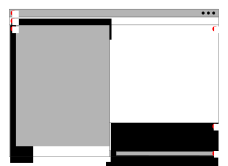
\includegraphics[width=\linewidth]{build/gui/main_view_initial.png}}
\captionof{figure}{Hauptfenster unmittelbar nach dem Starten des Programms}
\end{minipage}

Das Hauptfenster besteht aus der Fensterleiste (A), der Menüleiste (1), dem Editor (2), der Visualisierungsbox (3), der Konsole (4) und dem Eingabefeld (5).
Dabei ist die Fensterleiste kein Bestandteil des Programms; sie ist von der graphischen Oberfläche des Betriebssystems vorgegeben.
Das Eingabefeld ist deaktiviert (angedeutet durch die graue Färbung), da noch kein Prolog-Programm geparst wurde.

\subsubsection{\enquote{Datei}-Menü}

\begin{minipage}{\linewidth}
\makebox[\linewidth]{
    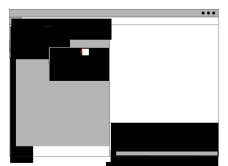
\includegraphics[width=\linewidth]{build/gui/main_view_filemenu.png}}
\captionof{figure}{Hauptfenster mit ausgewähltem \enquote{Datei}-Menü}
\end{minipage}

Das \enquote{Datei}-Menü (1) hat die Einträge \enquote{Neu}, \enquote{Öffnen}, \enquote{Speichern}, \enquote{Speichern als...}, \enquote{Zuletzt verwendet} und \enquote{Beenden}.
\enquote{Neu}, \enquote{Öffnen} und \enquote{Speichern} führen die jeweiligen Funktionen aus.
Während \enquote{Speichern} nur bei neu angelegten Prolog-Programmen einen Auswahldialog anzeigt, zeigt \enquote{Speichern als...} immer einen Auswahldialog an.
\enquote{Beenden} beendet das Programm.
\enquote{Zuletzt verwendet} enthält eine Liste von bis zu fünf zuletzt verwendeten Programmen (2).

\subsubsection{Geöffnete Datei}

\begin{minipage}{\linewidth}
\makebox[\linewidth]{
    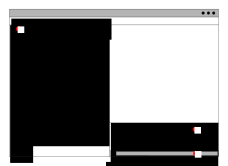
\includegraphics[width=\linewidth]{build/gui/main_view_opened.png}}
\captionof{figure}{Hauptfenster nach dem Öffnen des Beispielprogramms}
\end{minipage}

Nach dem Öffnen des Beispielprogramms wird dessen Inhalt im Editor angezeigt (1).
Die Konsole gibt eine entsprechende Meldung aus (2).
Das Eingabefeld bleibt weiterhin deaktiviert (3).

\subsubsection{Parsen fehlgeschlagen}

\begin{minipage}{\linewidth}
\makebox[\linewidth]{
    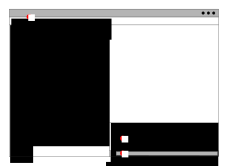
\includegraphics[width=\linewidth]{build/gui/main_view_parse_fail.png}
}
\captionof{figure}{Hauptfenster nach Klick auf \enquote{Parsen}, mit inkorrektem Prolog-Programm}
\end{minipage}

Klickt der Nutzer auf \enquote{Parsen} im \enquote{Programm}-Menü (1), versucht der Parser das Prolog-Programm im Editor zu verarbeiten.
Stößt er dabei auf Fehler, wird eine Fehlermeldung in der Konsole angezeigt (2).
Das Eingabefeld bleibt weiterhin deaktiviert (3).

\subsubsection{Parsen erfolgreich}

\begin{minipage}{\linewidth}
\makebox[\linewidth]{

\includegraphics[width=\linewidth]{build/gui/main_view_parse_success.png}
}
\captionof{figure}{Hauptfenster nach Klick auf \enquote{Parsen}, mit korrektem Prolog-Programm}
\end{minipage}

Klickt der Nutzer auf \enquote{Parsen} (1), versucht der Parser das Prolog-Programm im Editor zu verarbeiten.
Treten dabei keine Fehler auf, wird eine entsprechende Meldung in der Konsole angezeigt (2).
Das Eingabefeld wird aktiviert; der Nutzer kann jetzt Abfragen eingeben (3).

\subsection{Inkorrekte Abfrage}

\begin{minipage}{\linewidth}
\makebox[\linewidth]{

\includegraphics[width=\linewidth]{build/gui/main_view_question_fail.png}
}
\captionof{figure}{Hauptfenster nach inkorrekter Abfrage im Eingabefeld}
\end{minipage}

Gibt der Nutzer eine Abfrage im Eingabefeld ein (1), versucht der Parser, diese Eingabe zu einem einzelnen Ziel zu verarbeiten.
Stößt er dabei auf Fehler, wird eine Fehlermeldung in der Konsole angezeigt (2).

\subsubsection{Erfolgreiche Abfrage}

\begin{minipage}{\linewidth}
\makebox[\linewidth]{
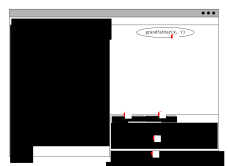
\includegraphics[width=\linewidth]{build/gui/main_view_visualisation_root.png}
}
\captionof{figure}{Hauptfenster nach Eingabe einer Abfrage}
\end{minipage}

Gibt der Nutzer eine Abfrage (1) im Eingabefeld ein, versucht der Parser, diese Eingabe zu einem einzelnen Ziel zu verarbeiten.
Treten dabei keine Fehler auf, wird eine Meldung in der Konsole angezeigt (2) und die Visualisierung der Abarbeitung dieser Abfrage gestartet (3).
Eine Leiste mit Schaltflächen, die zur Steuerung der Visualisierung dienen, wird angezeigt.
Die Schaltfäche \enquote{Nächster Schritt} (4) bewirkt die Ausführung und Visualisierung des nächsten Schrittes.
Die Schaltflächen \enquote{+} und \enquote{-} (5) dienen zum Zoomen in der Visualisierung.

\subsubsection{Lösung gefunden}

\begin{minipage}{\linewidth}
\makebox[\linewidth]{
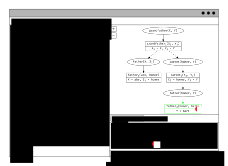
\includegraphics[width=\linewidth]{build/gui/main_view_solution_found.png}
}
\captionof{figure}{Eine Lösung wurde gefunden}
\end{minipage}

Wurde ein Lösung für die Abfrage gefunden (1), wird eine Meldung in der Konsole angezeigt (2).

\subsubsection{Keine weiteren Lösungen}

\begin{minipage}{\linewidth}
\makebox[\linewidth]{
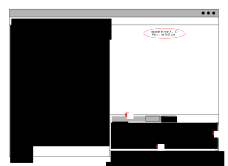
\includegraphics[width=\linewidth]{build/gui/main_view_no_more_solutions.png}
}
\captionof{figure}{Es gibt keine weiteren Lösungen mehr}
\end{minipage}

Gibt es keine weiteren Lösungen mehr, wird eine Meldung (1) in der Konsole angezeigt und die Schaltfläche \enquote{Nächster Schritt} wird deaktiviert (2).

Dieser Fall tritt ein, wenn der Interpreter einen Rückschritt vom eingegeben Ziel auszuführen versucht.
In diesem Fall gibt es keine Fakten mehr, die mit dem Ziel unifizierbar sind.
Unabhängig davon, ob es per se keine Lösungen gibt oder schon Lösungen gefunden wurden, wird die Meldung \enquote{Keine weiteren Lösungen.} angezeigt.

In diesem Entwurf ist außerdem der Scrollbalken gezeigt (3).
Dieser wird neben der Konsole eingeblendet, wenn der angezeigt Text nicht mehr hineinpasst.
Dies gilt auch für den Editor.

\subsection{Kannkriterien}

Jeder der folgenden Entwürfe beinhaltet \emph{ein} Kannkriterium.

\subsubsection{Schaltfläche \enquote{Vorheriger Schritt}}

\begin{minipage}{\linewidth}
\makebox[\linewidth]{
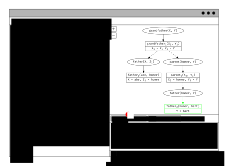
\includegraphics[width=\linewidth]{build/gui/main_view_previous_step.png}
}
    \captionof{figure}{Die Schaltfläche \enquote{vorheriger Schritt}}
\end{minipage}

\begin{minipage}{\linewidth}
\makebox[\linewidth]{
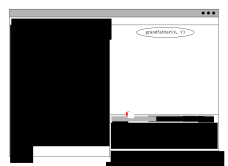
\includegraphics[width=\linewidth]{build/gui/main_view_previous_step_disabled.png}
}
\captionof{figure}{Interpreter beim ersten Schritt; die Schaltfläche \enquote{Vorheriger Schritt} ist deaktiviert}
\end{minipage}

Die Schaltfläche \enquote{Vorheriger Schritt} (1) erlaubt es dem Nutzer, den Zustand vor dem aktuellen Schritt zu betrachten.
Die Schaltfläche kann so lange betätigt werden, bis der Nutzer beim ersten Schritt angelangt ist.
Ist der Nutzer beim ersten Schritt angelangt, wird die Schaltfläche deaktiviert.

\subsubsection{Ausführung bis zur nächsten Lösung}

\begin{minipage}{\linewidth}
\makebox[\linewidth]{
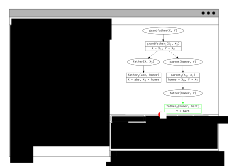
\includegraphics[width=\linewidth]{build/gui/main_view_next_solution.png}
}
\captionof{figure}{Die Schaltfläche \enquote{Nächste Lösung}}
\end{minipage}

\begin{minipage}{\linewidth}
\makebox[\linewidth]{
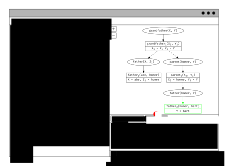
\includegraphics[width=\linewidth]{build/gui/main_view_abort.png}
}
\captionof{figure}{Die Schaltfläche \enquote{Abbrechen}}
\end{minipage}

Die Schaltfläche \enquote{Nächste Lösung} (1) lässt den Interpreter automatisch Schritte ausführen, bis eine Lösung gefunden wurde oder keine Unifikation der Abfrage mehr möglich ist.
Betätigt der Nutzer die Schaltfläche, wird sie hervorgehoben und ihr Text in \enquote{Abbrechen} geändert.
Betätigt der Nutzer die Schaltfläche erneut, wird der Interpreter nach der aktuellen Berechnung unterbrochen und der resultierende Zustand wird visualisiert.

\subsubsection{Export der Visualisierung}

\begin{minipage}{\linewidth}
\makebox[\linewidth]{
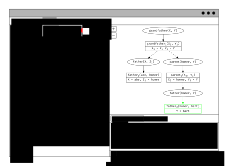
\includegraphics[width=\linewidth]{build/gui/main_view_exportmenu.png}
}
\captionof{figure}{Die Schaltflächen \enquote{Exportieren...}}
\end{minipage}

Die Schaltflächen \enquote{Exportieren als Bild} und \enquote{Exportieren als TikZ} erlauben dem Nutzer das Exportieren des Visualisierungsgraphen in verschiedenen Formaten (1).
\enquote{Exportieren als Bild} lässt den Nutzer zwischen dem Export als SVG- oder PNG-Graphik wählen.
\enquote{Exportieren als TikZ} lässt den Nutzer eine TeX-Datei mit einer Umsetzung des Graphen als TikZ-Graphik erstellen.

\subsubsection{Formatieren eines Prolog-Programms}

\begin{minipage}{\linewidth}
\makebox[\linewidth]{
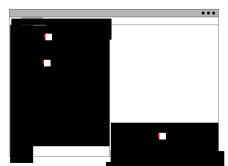
\includegraphics[width=\linewidth]{build/gui/main_view_format_button.png}
}
\captionof{figure}{Programm nach dem Betätigen der \enquote{Formatieren}-Schaltflfäche}
\end{minipage}

Wenn der Nutzer die Schaltfläche \enquote{Formatieren} betätigt, versucht das Programm, das Prolog-Programm im Editor nach den vorgegegeben Regeln zu formatieren.
Ist dies erfolgreich, wird eine Meldung auf der Konsole ausgegeben (2) und der Inhalt des Editors mit dem formatierten Prolog-Programm überschrieben (3).

Schlägt die Formatierung fehl, wird eine Fehlermeldung auf der Konsole ausgegeben.

\subsubsection{Schnellzugriffsleiste}

\begin{minipage}{\linewidth}
\makebox[\linewidth]{
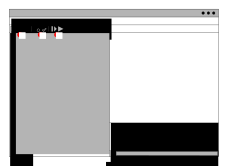
\includegraphics[width=\linewidth]{build/gui/main_view_buttonbar.png}
}
\captionof{figure}{Position der Schnellzugriffsleiste}
\end{minipage}

Die Schnellzugriffleiste bietet dem Nutzer die wichtigsten Funktionen an einem Ort.
Diese werden durch Schaltflächen mit Symbolen repräsentiert.
Die Symbole stehen für das Erstellen, Öffnen und Speichern von Dateien (1), Parsen und Formatieren von Prolog-Programmen (2) und \enquote{Ausführung eines Einzelschritts} sowie \enquote{Ausführung bis zur nächsten Lösung} (3).
Die Schaltflächen sind dabei nur aktiv, wenn auch ihre Gegenstücke an anderen Stellen in der GUI aktiv sind.
Im gezeigten Zustand sind die Schrittschaltflächen inaktiv, da kein prolog-Programm erfolgreich geparst wurde.

\subsection{Visualisierung}

Um die Visualisierungsbeispiele besser darzustellen zu können, wurden sie hier ohne die graphische Oberfläche des Programms eingefügt.
Die visualisierte Abfrage ist \texttt{grandfather(X, Y)} im Beispielprogramm.

\subsubsection{Wurzel}

\begin{minipage}{\linewidth}
\makebox[\linewidth]{
\includegraphics[width=0.7\linewidth]{build/visualisation/01_root.png}
}
\captionof{figure}{Wurzel des Visualisierungsbaumes}
\end{minipage}

Die Wurzel des Visualisierungsbaumes stellt die eingegebene Abfrage dar.

\subsubsection{Erfolgreiche Unifikation und Teilziele}

Die erste Regel mit zu \texttt{grandfather(X, Y)} passendem Funktornamen ist auch die einzige, in Zeile 6.
Die Unifikation mit dieser Regel ist erfolgreich.
Dabei werden die Variablennamen durch neue, eindeutige Namen ersetzt um Konflikte zu vermeiden.
Der neue Name einer Variable setzt sich zusammen aus dem ursprünglichen Namen und der laufenden Nummer der erfolgreichen Unifikation, beginnend bei eins.

\begin{minipage}{\linewidth}
\makebox[\linewidth]{
\includegraphics[width=\linewidth]{build/visualisation/03_root_success.png}
}
\captionof{figure}{Eine erfolgreiche Unifikation mit Einfügung der Teilziele}
\end{minipage}

Die Visualisierung stellt zu unifizierende Ziele als Runde Knoten dar.
Unifikationen werden in  Rechtecken dargestellt, die in zwei weitere Rechtecke aufgeteilt sind.
Dabei enthält jede Unifikation im oberen Rechteck den Fakt, mit dem unifiziert werden soll.
Erfolgreiche Unifikationen enthalten im unteren Rechteck die resultierenden Substitutionen.
Außerdem sind sie grün eingefärbt.

War eine Unifikation mit einer Regel erfolgreich, so werden ihre Teilziele als neue Ziele, also runde Knoten, zum Graphen hinzugefügt.
Die Substitutionen werden in den Teilzielen angewendet und hervorgehoben.
Die Unifikation und ihre Teilziele werden durch gestrichelte Kanten verbunden.
Dadurch werden im Baum die Fälle \enquote{Ziel wurde unifiziert mit} und \enquote{Ziel ist Teilziel von Regel} unterschieden.

\subsubsection{Erfolgreiche Unifikation mit Substution in weiteren Teilzielen}

Im nächsten Schritt steigt der Interpreter in die Teilziele ab und versucht, von links nach rechts diese zu unifizieren.

\begin{minipage}{\linewidth}
\makebox[\linewidth]{
\includegraphics[width=\linewidth]{build/visualisation/04_subgoal_father_success.png}
}
\captionof{figure}{Eine erfolgreiche Unifikation Substitution im nächsten Teilziel}
\end{minipage}

In diesem Beispiel hat der gefundene Fakt keine Teilziele.
Trotzdem müssen die Substitutionen in der restlichen Teilzielen angewendet werden.
Die angewendeten Substitutionen werden dabei in den betreffenden Zielen hervorgehoben.

\subsubsection{Backtracking}

Hier wurden einige Schritte übersprungen.
Das zweite Teilziel wurde mit der ersten Definition von \texttt{parent(X, Y)} unifiziert.
Diese hat als Teilziel \texttt{mother(X, Y)}.
Mit der Belegung \texttt{X = homer} gibt es dafür aber keine Lösung.
Der Interpreter muss also nach einer alternativen Definition von \texttt{parent} suchen und dazu zurückspringen (\enquote{Backtracking}).

\begin{minipage}{\linewidth}
\makebox[\linewidth]{
\includegraphics[width=\linewidth]{build/visualisation/09_mother_backtrack.png}
}
\captionof{figure}{Rücksprung nachdem ein Ziel nicht erfüllbar ist}
\end{minipage}

Ein Rücksprung wird durch eine aus Punkten bestehende, rot eingefärbte Kante dargestellt.
Das nicht erfüllbare Teilziel wird ebenfalls rot eingefärbt und mit dem Text \enquote{Nicht erfüllbar!} ergänzt.

\subsubsection{Fehlgeschlagene Unifikation}

Nach dem Rücksprung findet der Interpreter die zweite \texttt{parent(X, Y)}-Regel, die das Teilziel \texttt{father(X, Y)} hat.
Mit den bisherigen Lösungen ist das neue Ziel \texttt{father(homer, Y)}.
Der Interpreter versucht, mit \texttt{father(abe, homer)} zu unifizieren, da der Funktorname übereinstimmt.
Diese Unifikation schlägt fehl.

\begin{minipage}{\linewidth}
\makebox[\linewidth]{
\includegraphics[width=\linewidth]{build/visualisation/11_subgoal_father_fail.png}
}
\captionof{figure}{Eine fehlgeschlagene Unifikation}
\end{minipage}

Fehlgeschlagene Unifikationen enthalten im unteren Rechteck den Satz \enquote{Unifikation fehlgeschlagen:} und den Grund des Fehlschlags.
Außerdem sind sie rot eingefärbt.

\section{Glossar}

\subsection{Allgemein}

\textbf{Programm}:
Das vorgestellte VIPER-Programm. Dies ist zu unterscheiden von Prolog-Programmen.

\textbf{Prolog-Programm}:
Prolog-Quelltext in Form von Dateien auf einem Speichermedium. Dies ist zu unterscheiden von dem Programm im Sinne des VIPER-Programms.

\textbf{Prolog-Teilsprache}:
Es gibt Identifier, Variablen und Zahlen die wie folgt notiert werden:

\begin{lstlisting}
id := [a-z][a-zA-Z0-9]*
var := [A-Z][a-zA-Z0-9]*
num := [0-9]+
\end{lstlisting}

Es gibt Terme welche sich aus obigem zusammensetzen:

\begin{lstlisting}
Term := Funktor | var | num
Funktor := id | id( Term{, Term}* )
\end{lstlisting}

Und zusätzlich gibt es Regeln und Ziele welche sich wie folgt zusammensetzen:

\begin{lstlisting}
Regel := Funktor . | Funktor :- Ziel {, Ziel}* .
Ziel := Funktor | Term = Term
\end{lstlisting}

Außerdem unterstützt das Programm Listen.

\subsection{Prolog-interne Begriffe}
\textbf{Abfrage}:
Ziel, für das alle möglichen Lösungen gefunden werden sollen. Die Lösung kann eine Menge an Belegungen für Variablen oder eine Ja-Nein-Antwort sein.

\textbf{Arithmetik}:
Grundlegende Arithmetik beinhaltet natürliche Zahlen inklusive der 0. Des weiteren werden folgende Operatoren unterstützt:\\
\texttt{+, -, *, <, =<, >, >=, =\=, =:=}\\
\\
Da Termgleichheit in Prolog keine Arithmetik unterstützt, können Abfragen wie\\
\enquote{$4 = 1 + 3$}\\
nicht ausgewertet werden. Deshalb wird zusätzlicher der \texttt{is}-Operator unterstützt. Dieser evaluiert zuerst die rechte Seite arithmetisch und unifiziert diese anschließend mit der Linken.

\textbf{Backtracking / Rückschreiten}:
Aufheben der letzten Wahl bei der Suche nach einer passenden Variablenbelegung.

\textbf{Cut}:
Wird durch \enquote{\texttt{!}} dargestellt. Teilziel einer Regel, bei dem die erste Unifikation immer erfolgreich ist. Alle weiteren Unifikationen beim Backtracking schlagen fehl. Außerdem werden alle nachfolgenden Regeln mit dem selben Kopf verworfen.

\textbf{Fakt}:
Aussage, welche als wahr angenommen wird. Im Kontext von Prolog: eine Regel ohne Teilziele.

\textbf{Funktor}:
Sammelbegriff für einen einzelnen Identifier und Identifier in Kombination mit einer beliebigen Anzahl Termen, welche in Klammern hinter dem Identifier stehen.

\textbf{Gleichheit}:
Terme sind genau dann gleich, wenn die linke und rechte Seite eines Terms identisch sind oder wenn Variablen in den Termen so belegt werden können, dass beide Seiten identisch sind.

\textbf{Identifier}:
Wort, beginnend mit einem Kleinbuchstaben und fortsetzend mit Groß- und Kleinbuchstaben sowie Zahlen.

\textbf{Interpreter}:
Ausführungsmechanismus für Abfragen. Nachdem sowohl das zugrunde liegende Prolog-Programm als auch die Abfrage durch den Parser verarbeitet wurden, findet eine schrittweise Interpretation der genannten Abfrage statt.

\textbf{Listen}:
Die leere Liste wird durch \enquote{\texttt{[]}} dargestellt. Eine Liste mit Inhalt wird durch \enquote{\texttt{[1,2,3]}} dargestellt und intern als Listenkopf und \enquote{Restliste} behandelt, das heißt:\\
\texttt{[1,2,3]} =\\
\texttt{[1|Teilliste1], Teilliste1=[2|Teilliste2], Teilliste2=[3|[]]} =\\
\texttt{[1|[2|[3|[]]]]}

\textbf{Parser}:
Umwandlungsmechanismus für Prolog-Programme, der diese in ein für die Weiterverarbeitung geeignetes Format bringt und auf syntaktische Fehler prüft.

\textbf{Regel}:
Vorgeschriebene Folgerungen. Regeln können bspw. festsetzen, dass aus dem Fakt, dass jemand ein Elternteil ist, folgt, dass dieser Elternteil entweder Mutter oder Vater sein muss.

\textbf{Schritt}:
Nächste Operation, die zur Interpretation einer Abfrage nötig ist.

\textbf{Standardbibliothek}:
Voreingestellte Regeln, welche automatisch bei der Verarbeitung durch den Parser angefügt werden können.

\textbf{Term}:
Sammelbegriff für Funktoren, Variablen oder Zahlen.

\textbf{Unifikation}:
Zwei Terme sind genau dann unifizierbar, wenn sie gleich sind oder Variablen enthalten, die so belegt werden können dass die Terme gleich sind.

\textbf{Variable}:
Platzhalter. Erlaubt das allgemeine Beschreiben von Regeln. Können für einen beliebigen Term stehen.

\textbf{Ziel}:
Lösbarer Teil einer Regel, welcher einem Funktor, einem Unifikationsziel, Arithmetik oder dem \enquote{Cut}-Operator entsprechen kann.

\textbf{Zustand}:
Ergebnis der bisher durchgeführten Schritte.

\textbf{Zustandsunterschied}:
Schritte zwischen zwei Zuständen.

\subsection{Begriffe der Bedienoberfläche}
\textbf{Dialog}:
Fenster zur Meldung einer Nachricht (Warnungs- oder Fehler-Dialog) oder Anfrage (bspw. Bestätigungs-Dialog).

\textbf{Editor}:
Element der graphischen Oberfläche, welches Eingabe und Bearbeitung von angezeigtem Text ermöglicht.

\textbf{Eingabefeld}:
Element der graphischen Oberfläche. Das Eingabefeld dient zur Eingabe von Abfragen. Es ist nur dann aktiviert, wenn ein korrektes Prolog-Programm eingegeben und geparst wurde.

\textbf{Export}:
Schreiben von Bild-Dateien oder LaTeX-Quellcode in ein Zielverzeichnis auf einem verbundenen Speichermedium. Das Schreiben von Prolog-Programmen auf ein Speichermedium wird nicht als Export, sondern als Speichern bezeichnet.

\textbf{Formatierung}:
Vorgegebener Stil bzgl. der Setzung von Leerzeichen und Umbrüchen. Zu unterscheiden von Syntax, da Formatierung keinen Einfluss auf die Validität des Programms hat.

\textbf{Graph}:
Struktur bestehend aus Knoten und Kanten.

\textbf{GUI / GUI-Element}:
Das GUI entspricht der graphischen Benutzeroberfläche (graphical user interface). Das GUI ist zusammengesetzt aus diversen GUI-Elementen innerhalb eines Fensters (bspw. dem Editor).

\textbf{Konsole}:
Element der graphischen Oberfläche. Die Konsole ist nur lesbar und dient der Ausgabe von Ergebnissen einer Abfrage sowie anderen Meldungen. 

\textbf{Menüleiste}:
Element der graphischen Oberfläche. Bietet über Text-Menüs Zugriff auf Funktionen wie Speichern und Öffnen.

\textbf{Öffnen}:
Lesen eines ausgewählten Prolog-Programms von einem verbundenen Speichermedium in das Programm. Dies entspricht der Übertragung des Textes aus der gewählten Datei in den Editor.

\textbf{Speichern}:
Schreiben einer Prolog-Programmdatei in ein Zielverzeichnis auf einem verbundenen Speichermedium. Es werden ausschließlich Prolog-Programme gespeichert, andere Schreibvorgänge auf Speichermedien fallen unter den Begriff Export.

\textbf{Visualisierung}:
Navigierbarer Graph, welcher den Ablauf der Interpretation einer Abfrage im Kontext eines gegebenen Prolog-Programms aufzeigt.

\textbf{Zoom}:
Vergrößerung oder Verkleinerung eines Bildausschnitts.

\newpage
\section{Anhang}

\subsection{Unformatiertes simpsons.pl Beispielprogramm}

\begin{lstlisting}
father(abe, homer). father(homer, bart).
father(homer, lisa). mother(marge, bart).

grandfather(X, Y) :-
father(X, Z), parent(Z, Y).

parent(X, Y) :- mother(X, Y).

parent(X, Y) :- father(X, Y).
\end{lstlisting}

\subsection{Formatiertes \texttt{simpsons.pl} Beispielprogramm}

\begin{lstlisting}
father(abe, homer).
father(homer, bart).
father(homer, lisa).
mother(marge, bart).

grandfather(X, Y) :-
  father(X, Z),
  parent(Z, Y).

parent(X, Y) :-
  mother(X, Y).

parent(X, Y) :-
  father(X, Y).
\end{lstlisting}

\end{document}
